% Created by tikzDevice version 0.12.3.1 on 2021-07-01 17:33:03
% !TEX encoding = UTF-8 Unicode
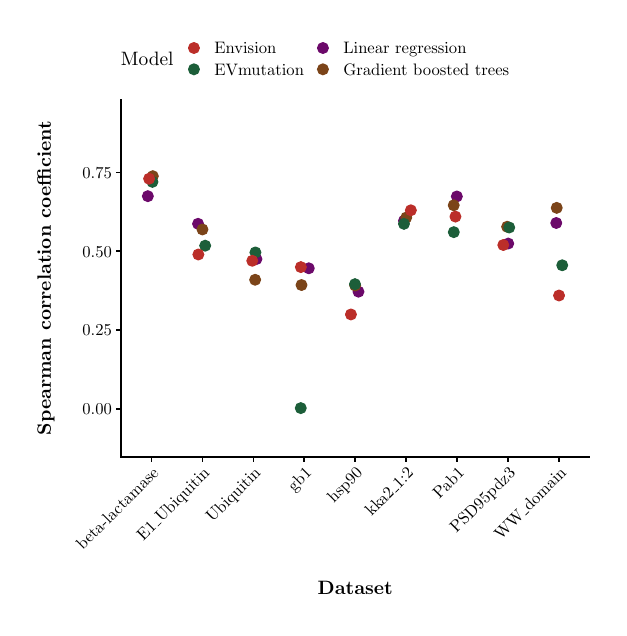
\begin{tikzpicture}[x=1pt,y=1pt]
\definecolor{fillColor}{RGB}{255,255,255}
\path[use as bounding box,fill=fillColor,fill opacity=0.00] (0,0) rectangle (206.56,209.59);
\begin{scope}
\path[clip] ( 33.67, 54.47) rectangle (203.06,183.69);
\definecolor{drawColor}{RGB}{108,9,106}
\definecolor{fillColor}{RGB}{108,9,106}

\path[draw=drawColor,line width= 0.4pt,line join=round,line cap=round,fill=fillColor] ( 43.42,148.70) circle (  1.96);
\definecolor{drawColor}{RGB}{123,68,25}
\definecolor{fillColor}{RGB}{123,68,25}

\path[draw=drawColor,line width= 0.4pt,line join=round,line cap=round,fill=fillColor] ( 45.22,155.93) circle (  1.96);
\definecolor{drawColor}{RGB}{28,94,57}
\definecolor{fillColor}{RGB}{28,94,57}

\path[draw=drawColor,line width= 0.4pt,line join=round,line cap=round,fill=fillColor] ( 45.08,153.86) circle (  1.96);
\definecolor{drawColor}{RGB}{108,9,106}
\definecolor{fillColor}{RGB}{108,9,106}

\path[draw=drawColor,line width= 0.4pt,line join=round,line cap=round,fill=fillColor] ( 61.57,138.72) circle (  1.96);
\definecolor{drawColor}{RGB}{123,68,25}
\definecolor{fillColor}{RGB}{123,68,25}

\path[draw=drawColor,line width= 0.4pt,line join=round,line cap=round,fill=fillColor] ( 63.16,136.68) circle (  1.96);
\definecolor{drawColor}{RGB}{28,94,57}
\definecolor{fillColor}{RGB}{28,94,57}

\path[draw=drawColor,line width= 0.4pt,line join=round,line cap=round,fill=fillColor] ( 64.14,130.81) circle (  1.96);
\definecolor{drawColor}{RGB}{108,9,106}
\definecolor{fillColor}{RGB}{108,9,106}

\path[draw=drawColor,line width= 0.4pt,line join=round,line cap=round,fill=fillColor] ( 82.66,125.98) circle (  1.96);
\definecolor{drawColor}{RGB}{123,68,25}
\definecolor{fillColor}{RGB}{123,68,25}

\path[draw=drawColor,line width= 0.4pt,line join=round,line cap=round,fill=fillColor] ( 82.20,118.49) circle (  1.96);
\definecolor{drawColor}{RGB}{28,94,57}
\definecolor{fillColor}{RGB}{28,94,57}

\path[draw=drawColor,line width= 0.4pt,line join=round,line cap=round,fill=fillColor] ( 82.30,128.37) circle (  1.96);
\definecolor{drawColor}{RGB}{108,9,106}
\definecolor{fillColor}{RGB}{108,9,106}

\path[draw=drawColor,line width= 0.4pt,line join=round,line cap=round,fill=fillColor] (101.58,122.64) circle (  1.96);
\definecolor{drawColor}{RGB}{123,68,25}
\definecolor{fillColor}{RGB}{123,68,25}

\path[draw=drawColor,line width= 0.4pt,line join=round,line cap=round,fill=fillColor] ( 98.95,116.59) circle (  1.96);
\definecolor{drawColor}{RGB}{28,94,57}
\definecolor{fillColor}{RGB}{28,94,57}

\path[draw=drawColor,line width= 0.4pt,line join=round,line cap=round,fill=fillColor] ( 98.68, 72.12) circle (  1.96);
\definecolor{drawColor}{RGB}{108,9,106}
\definecolor{fillColor}{RGB}{108,9,106}

\path[draw=drawColor,line width= 0.4pt,line join=round,line cap=round,fill=fillColor] (119.53,114.19) circle (  1.96);
\definecolor{drawColor}{RGB}{123,68,25}
\definecolor{fillColor}{RGB}{123,68,25}

\path[draw=drawColor,line width= 0.4pt,line join=round,line cap=round,fill=fillColor] (118.34,116.42) circle (  1.96);
\definecolor{drawColor}{RGB}{28,94,57}
\definecolor{fillColor}{RGB}{28,94,57}

\path[draw=drawColor,line width= 0.4pt,line join=round,line cap=round,fill=fillColor] (118.27,116.91) circle (  1.96);
\definecolor{drawColor}{RGB}{108,9,106}
\definecolor{fillColor}{RGB}{108,9,106}

\path[draw=drawColor,line width= 0.4pt,line join=round,line cap=round,fill=fillColor] (135.98,139.82) circle (  1.96);
\definecolor{drawColor}{RGB}{123,68,25}
\definecolor{fillColor}{RGB}{123,68,25}

\path[draw=drawColor,line width= 0.4pt,line join=round,line cap=round,fill=fillColor] (136.81,140.98) circle (  1.96);
\definecolor{drawColor}{RGB}{28,94,57}
\definecolor{fillColor}{RGB}{28,94,57}

\path[draw=drawColor,line width= 0.4pt,line join=round,line cap=round,fill=fillColor] (135.97,138.70) circle (  1.96);
\definecolor{drawColor}{RGB}{108,9,106}
\definecolor{fillColor}{RGB}{108,9,106}

\path[draw=drawColor,line width= 0.4pt,line join=round,line cap=round,fill=fillColor] (155.08,148.60) circle (  1.96);
\definecolor{drawColor}{RGB}{123,68,25}
\definecolor{fillColor}{RGB}{123,68,25}

\path[draw=drawColor,line width= 0.4pt,line join=round,line cap=round,fill=fillColor] (153.95,145.41) circle (  1.96);
\definecolor{drawColor}{RGB}{28,94,57}
\definecolor{fillColor}{RGB}{28,94,57}

\path[draw=drawColor,line width= 0.4pt,line join=round,line cap=round,fill=fillColor] (153.98,135.70) circle (  1.96);
\definecolor{drawColor}{RGB}{108,9,106}
\definecolor{fillColor}{RGB}{108,9,106}

\path[draw=drawColor,line width= 0.4pt,line join=round,line cap=round,fill=fillColor] (173.65,131.58) circle (  1.96);
\definecolor{drawColor}{RGB}{123,68,25}
\definecolor{fillColor}{RGB}{123,68,25}

\path[draw=drawColor,line width= 0.4pt,line join=round,line cap=round,fill=fillColor] (173.25,137.65) circle (  1.96);
\definecolor{drawColor}{RGB}{28,94,57}
\definecolor{fillColor}{RGB}{28,94,57}

\path[draw=drawColor,line width= 0.4pt,line join=round,line cap=round,fill=fillColor] (174.01,137.38) circle (  1.96);
\definecolor{drawColor}{RGB}{108,9,106}
\definecolor{fillColor}{RGB}{108,9,106}

\path[draw=drawColor,line width= 0.4pt,line join=round,line cap=round,fill=fillColor] (191.01,139.01) circle (  1.96);
\definecolor{drawColor}{RGB}{123,68,25}
\definecolor{fillColor}{RGB}{123,68,25}

\path[draw=drawColor,line width= 0.4pt,line join=round,line cap=round,fill=fillColor] (191.17,144.48) circle (  1.96);
\definecolor{drawColor}{RGB}{28,94,57}
\definecolor{fillColor}{RGB}{28,94,57}

\path[draw=drawColor,line width= 0.4pt,line join=round,line cap=round,fill=fillColor] (193.16,123.73) circle (  1.96);
\definecolor{drawColor}{RGB}{187,46,41}
\definecolor{fillColor}{RGB}{187,46,41}

\path[draw=drawColor,line width= 0.4pt,line join=round,line cap=round,fill=fillColor] ( 43.88,155.00) circle (  1.96);

\path[draw=drawColor,line width= 0.4pt,line join=round,line cap=round,fill=fillColor] (154.57,141.32) circle (  1.96);

\path[draw=drawColor,line width= 0.4pt,line join=round,line cap=round,fill=fillColor] ( 61.68,127.63) circle (  1.96);

\path[draw=drawColor,line width= 0.4pt,line join=round,line cap=round,fill=fillColor] (138.46,143.60) circle (  1.96);

\path[draw=drawColor,line width= 0.4pt,line join=round,line cap=round,fill=fillColor] (171.87,131.05) circle (  1.96);

\path[draw=drawColor,line width= 0.4pt,line join=round,line cap=round,fill=fillColor] (192.01,112.81) circle (  1.96);

\path[draw=drawColor,line width= 0.4pt,line join=round,line cap=round,fill=fillColor] ( 81.16,125.35) circle (  1.96);

\path[draw=drawColor,line width= 0.4pt,line join=round,line cap=round,fill=fillColor] ( 98.72,123.07) circle (  1.96);

\path[draw=drawColor,line width= 0.4pt,line join=round,line cap=round,fill=fillColor] (116.81,105.96) circle (  1.96);
\end{scope}
\begin{scope}
\path[clip] (  0.00,  0.00) rectangle (206.56,209.59);
\definecolor{drawColor}{RGB}{0,0,0}

\path[draw=drawColor,line width= 0.6pt,line join=round,line cap=rect] ( 33.67, 54.47) --
	( 33.67,183.69);
\end{scope}
\begin{scope}
\path[clip] (  0.00,  0.00) rectangle (206.56,209.59);
\definecolor{drawColor}{RGB}{0,0,0}

\node[text=drawColor,anchor=base east,inner sep=0pt, outer sep=0pt, scale=  0.60] at ( 30.42, 69.68) {0.00};

\node[text=drawColor,anchor=base east,inner sep=0pt, outer sep=0pt, scale=  0.60] at ( 30.42, 98.19) {0.25};

\node[text=drawColor,anchor=base east,inner sep=0pt, outer sep=0pt, scale=  0.60] at ( 30.42,126.71) {0.50};

\node[text=drawColor,anchor=base east,inner sep=0pt, outer sep=0pt, scale=  0.60] at ( 30.42,155.22) {0.75};
\end{scope}
\begin{scope}
\path[clip] (  0.00,  0.00) rectangle (206.56,209.59);
\definecolor{drawColor}{RGB}{0,0,0}

\path[draw=drawColor,line width= 0.6pt,line join=round] ( 31.92, 71.75) --
	( 33.67, 71.75);

\path[draw=drawColor,line width= 0.6pt,line join=round] ( 31.92,100.26) --
	( 33.67,100.26);

\path[draw=drawColor,line width= 0.6pt,line join=round] ( 31.92,128.77) --
	( 33.67,128.77);

\path[draw=drawColor,line width= 0.6pt,line join=round] ( 31.92,157.28) --
	( 33.67,157.28);
\end{scope}
\begin{scope}
\path[clip] (  0.00,  0.00) rectangle (206.56,209.59);
\definecolor{drawColor}{RGB}{0,0,0}

\path[draw=drawColor,line width= 0.6pt,line join=round,line cap=rect] ( 33.67, 54.47) --
	(203.06, 54.47);
\end{scope}
\begin{scope}
\path[clip] (  0.00,  0.00) rectangle (206.56,209.59);
\definecolor{drawColor}{RGB}{0,0,0}

\path[draw=drawColor,line width= 0.6pt,line join=round] ( 44.72, 52.72) --
	( 44.72, 54.47);

\path[draw=drawColor,line width= 0.6pt,line join=round] ( 63.13, 52.72) --
	( 63.13, 54.47);

\path[draw=drawColor,line width= 0.6pt,line join=round] ( 81.54, 52.72) --
	( 81.54, 54.47);

\path[draw=drawColor,line width= 0.6pt,line join=round] ( 99.95, 52.72) --
	( 99.95, 54.47);

\path[draw=drawColor,line width= 0.6pt,line join=round] (118.36, 52.72) --
	(118.36, 54.47);

\path[draw=drawColor,line width= 0.6pt,line join=round] (136.78, 52.72) --
	(136.78, 54.47);

\path[draw=drawColor,line width= 0.6pt,line join=round] (155.19, 52.72) --
	(155.19, 54.47);

\path[draw=drawColor,line width= 0.6pt,line join=round] (173.60, 52.72) --
	(173.60, 54.47);

\path[draw=drawColor,line width= 0.6pt,line join=round] (192.01, 52.72) --
	(192.01, 54.47);
\end{scope}
\begin{scope}
\path[clip] (  0.00,  0.00) rectangle (206.56,209.59);
\definecolor{drawColor}{RGB}{0,0,0}

\node[text=drawColor,rotate= 45.00,anchor=base east,inner sep=0pt, outer sep=0pt, scale=  0.60] at ( 47.64, 48.30) {beta-lactamase};

\node[text=drawColor,rotate= 45.00,anchor=base east,inner sep=0pt, outer sep=0pt, scale=  0.60] at ( 66.05, 48.30) {E1\_Ubiquitin};

\node[text=drawColor,rotate= 45.00,anchor=base east,inner sep=0pt, outer sep=0pt, scale=  0.60] at ( 84.46, 48.30) {Ubiquitin};

\node[text=drawColor,rotate= 45.00,anchor=base east,inner sep=0pt, outer sep=0pt, scale=  0.60] at (102.88, 48.30) {gb1};

\node[text=drawColor,rotate= 45.00,anchor=base east,inner sep=0pt, outer sep=0pt, scale=  0.60] at (121.29, 48.30) {hsp90};

\node[text=drawColor,rotate= 45.00,anchor=base east,inner sep=0pt, outer sep=0pt, scale=  0.60] at (139.70, 48.30) {kka2\_1:2};

\node[text=drawColor,rotate= 45.00,anchor=base east,inner sep=0pt, outer sep=0pt, scale=  0.60] at (158.11, 48.30) {Pab1};

\node[text=drawColor,rotate= 45.00,anchor=base east,inner sep=0pt, outer sep=0pt, scale=  0.60] at (176.52, 48.30) {PSD95pdz3};

\node[text=drawColor,rotate= 45.00,anchor=base east,inner sep=0pt, outer sep=0pt, scale=  0.60] at (194.93, 48.30) {WW\_domain};
\end{scope}
\begin{scope}
\path[clip] (  0.00,  0.00) rectangle (206.56,209.59);
\definecolor{drawColor}{RGB}{0,0,0}

\node[text=drawColor,anchor=base,inner sep=0pt, outer sep=0pt, scale=  0.70] at (118.36,  4.86) {\bfseries Dataset};
\end{scope}
\begin{scope}
\path[clip] (  0.00,  0.00) rectangle (206.56,209.59);
\definecolor{drawColor}{RGB}{0,0,0}

\node[text=drawColor,rotate= 90.00,anchor=base,inner sep=0pt, outer sep=0pt, scale=  0.70] at (  8.39,119.08) {\bfseries Spearman correlation coefficient};
\end{scope}
\begin{scope}
\path[clip] (  0.00,  0.00) rectangle (206.56,209.59);
\definecolor{drawColor}{RGB}{0,0,0}

\node[text=drawColor,anchor=base west,inner sep=0pt, outer sep=0pt, scale=  0.70] at ( 33.67,195.97) {Model};
\end{scope}
\begin{scope}
\path[clip] (  0.00,  0.00) rectangle (206.56,209.59);
\definecolor{drawColor}{RGB}{187,46,41}
\definecolor{fillColor}{RGB}{187,46,41}

\path[draw=drawColor,line width= 0.4pt,line join=round,line cap=round,fill=fillColor] ( 60.08,202.24) circle (  1.96);
\end{scope}
\begin{scope}
\path[clip] (  0.00,  0.00) rectangle (206.56,209.59);
\definecolor{drawColor}{RGB}{28,94,57}
\definecolor{fillColor}{RGB}{28,94,57}

\path[draw=drawColor,line width= 0.4pt,line join=round,line cap=round,fill=fillColor] ( 60.08,194.54) circle (  1.96);
\end{scope}
\begin{scope}
\path[clip] (  0.00,  0.00) rectangle (206.56,209.59);
\definecolor{drawColor}{RGB}{108,9,106}
\definecolor{fillColor}{RGB}{108,9,106}

\path[draw=drawColor,line width= 0.4pt,line join=round,line cap=round,fill=fillColor] (106.69,202.24) circle (  1.96);
\end{scope}
\begin{scope}
\path[clip] (  0.00,  0.00) rectangle (206.56,209.59);
\definecolor{drawColor}{RGB}{123,68,25}
\definecolor{fillColor}{RGB}{123,68,25}

\path[draw=drawColor,line width= 0.4pt,line join=round,line cap=round,fill=fillColor] (106.69,194.54) circle (  1.96);
\end{scope}
\begin{scope}
\path[clip] (  0.00,  0.00) rectangle (206.56,209.59);
\definecolor{drawColor}{RGB}{0,0,0}

\node[text=drawColor,anchor=base west,inner sep=0pt, outer sep=0pt, scale=  0.60] at ( 67.43,200.17) {Envision};
\end{scope}
\begin{scope}
\path[clip] (  0.00,  0.00) rectangle (206.56,209.59);
\definecolor{drawColor}{RGB}{0,0,0}

\node[text=drawColor,anchor=base west,inner sep=0pt, outer sep=0pt, scale=  0.60] at ( 67.43,192.47) {EVmutation};
\end{scope}
\begin{scope}
\path[clip] (  0.00,  0.00) rectangle (206.56,209.59);
\definecolor{drawColor}{RGB}{0,0,0}

\node[text=drawColor,anchor=base west,inner sep=0pt, outer sep=0pt, scale=  0.60] at (114.04,200.17) {Linear regression};
\end{scope}
\begin{scope}
\path[clip] (  0.00,  0.00) rectangle (206.56,209.59);
\definecolor{drawColor}{RGB}{0,0,0}

\node[text=drawColor,anchor=base west,inner sep=0pt, outer sep=0pt, scale=  0.60] at (114.04,192.47) {Gradient boosted trees};
\end{scope}
\end{tikzpicture}
